\documentclass[a4paper,10pt]{article}
\usepackage[a4paper, total={6in, 10in}]{geometry}
\usepackage[python,stopserver]{runcode}
%\usepackage[cache]{runcode}
\setminted[python]{fontsize=\footnotesize,linenos=false, frame=single, bgcolor=bg, breaklines=true}

% to compile it from scratch, create a generated subfolder and comment out the [cache] options below.
% Keep in mind that some steps take a few minutes to complete (to run the bootstrap)


\usepackage{caption}
%\usepackage{subcaption}
\usepackage{subfig}

% Title Page
\title{The betaMixPy package}
\author{Haim Bar}


\begin{document}
\maketitle

\section{Introduction}
The betaMixPy package is used to find edges in gene networks using co-expression data. The betaMix method is built on the insightful results of \cite{Frankl1990} who showed that two random vectors are approximately perpendicular with high probability, if the dimension of the space is sufficiently large. The pair-wise correlations between pairs of predictors are equal to the cosine of the angles between the pairs. From these angles we compute $z_j=\sin^2(\theta)$ and fit a mixture of two beta distributions. For pairs of random vectors (the null set) the distribution of $z_j$ is Beta((N-1)/2, 1/2), where N is the sample size. The nonnull set is assumed to follow a Beta(a,b) distribution, and using the EM algorithm we estimate a,b, and the proportion, $p_0$, of the null set of pairs. The betaMix function determines a threshold which will control the error rate given by the user. Any $z_j$ below that threshold corresponds to a significantly correlated pair of predictors (an edge in the graphical model.)
If the N samples can be assumed to be independent, set the parameter \texttt{ind} to True. If it is set to False, the null set follows a Beta(($\nu$-1)/2, 1/2) distribution and $\nu$ (the effective sample size) is estimated from the data.

The input to the program is a normalized expression matrix, with predictors/genes (which are the nodes in the graph) in the columns, and samples in the rows.

With a large number of predictors, P, the estimation may be slow, so it is recommended to set the parameter \texttt{subsamplesize} to something smaller than $P(P-1)/2$. The minimum allowed by the program is 20,000. Using anything smaller will cause betaMix to fit the model to all $P(P-1)/2$ pairs. 

The betaMix package requires the following Python packages: statistics, matplotlib, pandas, networkx, numpy, scipy.


\section{Simulated Data}
The data folder in this repository contains four simulated datasets as csv files:
\begin{enumerate}
\item \verb|cls_0200_1000_03_0050.csv|	contains 1000 predictors, and $N=200$ samples. The predictors come in 20 clusters, with 50 predictors in each cluster, such that the correlation of pairs within cluster is 0.3, and zero across clusters.
\item \verb|rbk_0500_0500_03.csv| Similar to the previous item, except that the clusters have random sizes, and $P=500$, and $N=500$.
\item \verb|hub_0500_0500_03_0025.csv| 	contains 500 predictors, and $N=500$ samples. The predictors are arranged as 25 hubs, so that each hub consists of 20 predictors of which one is the central node and all other nodes have a 0.3 correlation with it. The correlation of pairs across hubs is zero.
\item \verb|hub_0200_1000_09_0020.csv|	Similar to the previous item, except that $P=1000$, $N=200$ and the correlation between a central node and all other nodes in a hub is 0.9.
\end{enumerate}

We demonstrate the usage of the package with the first configuration (\texttt{i=0} in the code below).
\showCode{python}{../code/Simulated.py}[1][12]
Note that in line 9 we transpose the data matrix, since the betaMix method treats the data as $P$ vectors in an $R^N$. We set the null posterior probability threshold to \texttt{ppr=0.01}, and we set \texttt{subsamplesize=50000} which means that in the fitting process we take a random sample of size 50000 pairwise correlations, rather than using all $P(P-1)/2$ possible pairs. We also set \texttt{ind=True} so that  the N samples are assumed to be independent when we fit the model (in this case, the null distribution is determined exactly by the sample size).

\runPython{../code/Simulated.py}{sim}%[cache]
After fitting the model, we can obtain a summary of the parameter estimates and a plot of the fitted mixture distribution on top of the actual data histogram. This is done with the following code:
\showCode{python}{../code/Simulated.py}[13][14]

The model-fit summary in this case is summarized as follows:
\includeOutput{sim}[vbox]	

The fitted distribution plot is shown on the log-scale (Figure \ref{simFit}), where the null distribution is linear (depicted as a light blue line.) The nonnull component (shown in purple) is obtained from the estimates \texttt{ahat}, \texttt{bhat}, and \texttt{bmax} (the upper bound of the support of non-null component).  The red dotted line shows the cutoff, such that all the pairs which yield a $z_j$ statistic less than this threshold are considered nonnull. In this case, all the nonnull pairs were generated with the same correlation so the beta distribution fits the nonnull component very well but, in general it doesn't have to be this way -- the important thing is that for true nonnull pairs, the nonnull component will be much more likely than the null distribution. 

\begin{figure}[t!]
\centering
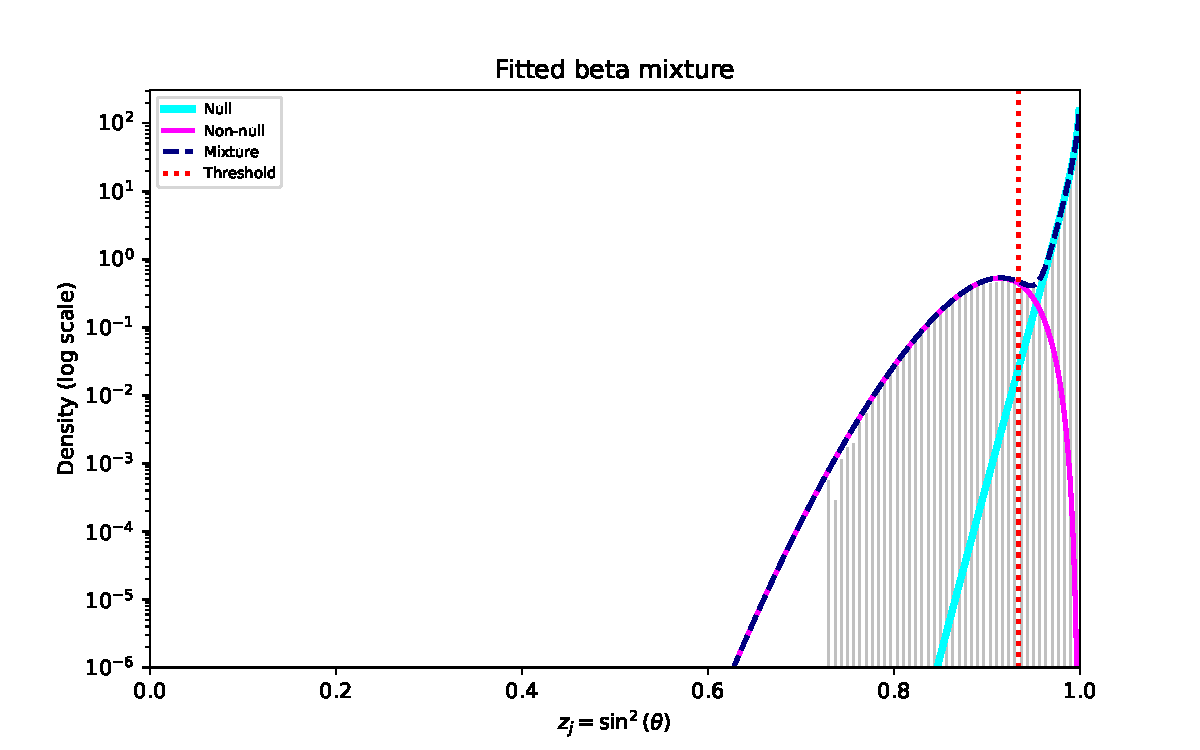
\includegraphics[width=.6\linewidth]{../figures/fitted.pdf}
\caption{Simulation 1 -- $N=200$, $P=1000$, 20 clusters with 50 predictors in each cluster, such that the true correlation of pairs within cluster is 0.3, and zero across clusters.}\label{simFit}
\end{figure}

In order to cluster the predictors we first have to generate the adjacency matrix and find graph components by running the following code
\showCode{python}{../code/Simulated.py}[16][17]

Then, we can show the pairwise correlations as a bitmap, as in Figure \ref{CorMatEst}. 
\showCode{python}{../code/Simulated.py}[18][18]
We can clearly see in Figure \ref{CorMatEst} that the algorithm detects the correct correlation structure (the yellow squares along the diagonal). The true correlation is modest ($\rho=0.3$) and $P=1000$ is quite large, and greater than $N=200$, but still, most of the true correlations are detected. In similar simulations, where either $\rho$ is greater, or $N$ is larger the true positive rate approaches 1. Furthermore, there are no yellow dots outside the diagonal of blocks, since our method yields an excellent false detection rate.
\begin{figure}[b!]
\centering
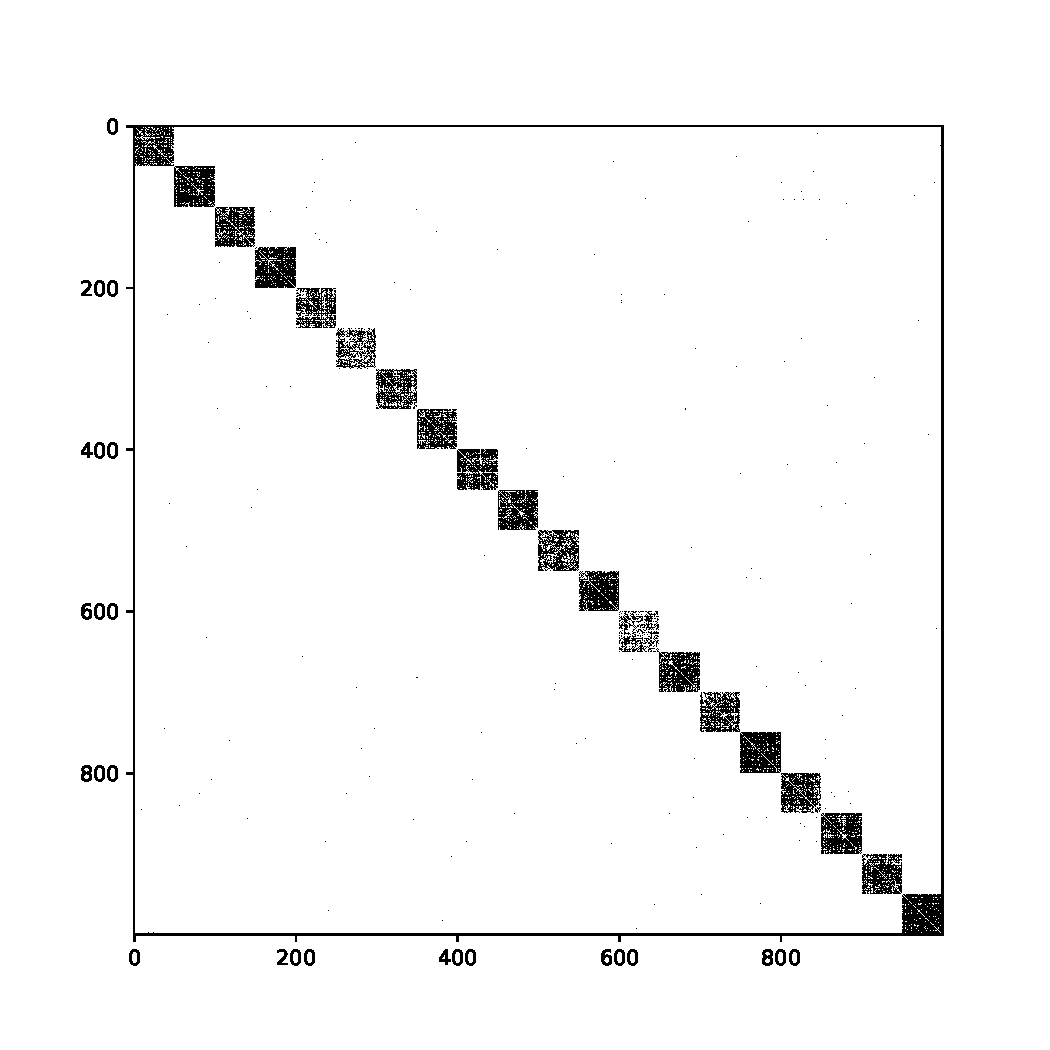
\includegraphics[width=.8\linewidth]{../figures/CorMatEst.pdf}
\caption{Simulation 1 -- the inferred adjacency matrix after fitting the betaMix model.}\label{CorMatEst}
\end{figure}

To visualize a certain cluster, we use the following code, which yields Figure \ref{Cluster}.
\showCode{python}{../code/Simulated.py}[20][20]

\begin{figure}[t!]
\centering
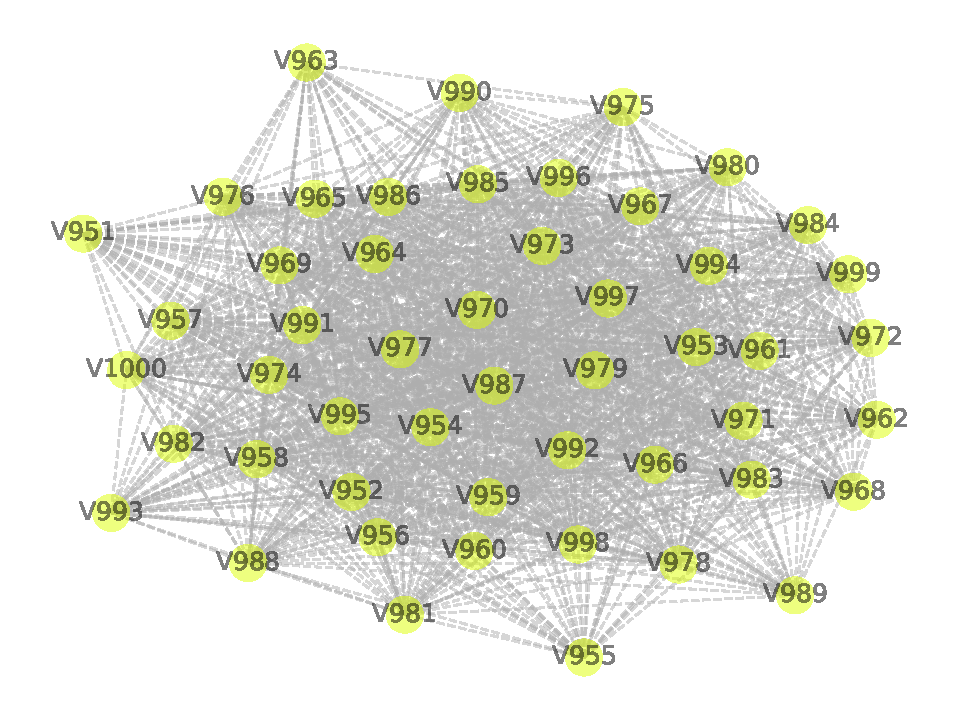
\includegraphics[width=.8\linewidth]{../figures/Cluster.pdf}
\caption{Simulation 1 -- cluster 1.}\label{Cluster}
\end{figure}


\section{Case Study -- Tomato Seeds}
We use the tomato metabolomic data from www.metabolomicsworkbench.org website, Study ID ST000561, introduced in \cite{tomatos2017}. There are two groups -- `dry seeds' and `six-hour imbibed seeds'. Each group has $n=50$, and a total of $P=68$ metabolites. We construct the metabolite network for each group separately. The code for the control (dry seeds) group is given below. The code for the second group is similar (and available in the GitHub repository.

\showCode{python}{../code/Tomatos.py}[1][10]
\runPython{../code/Tomatos.py}{sim}[cache]

Figure \ref{tomatos1} shows the bitmap representation of the two networks. The metabolites in the Dry Seed group are much less connected than in the Six-hour Imbibed group.

\begin{figure}[b!]
\centering
\subfloat[\centering Dry Seeds]{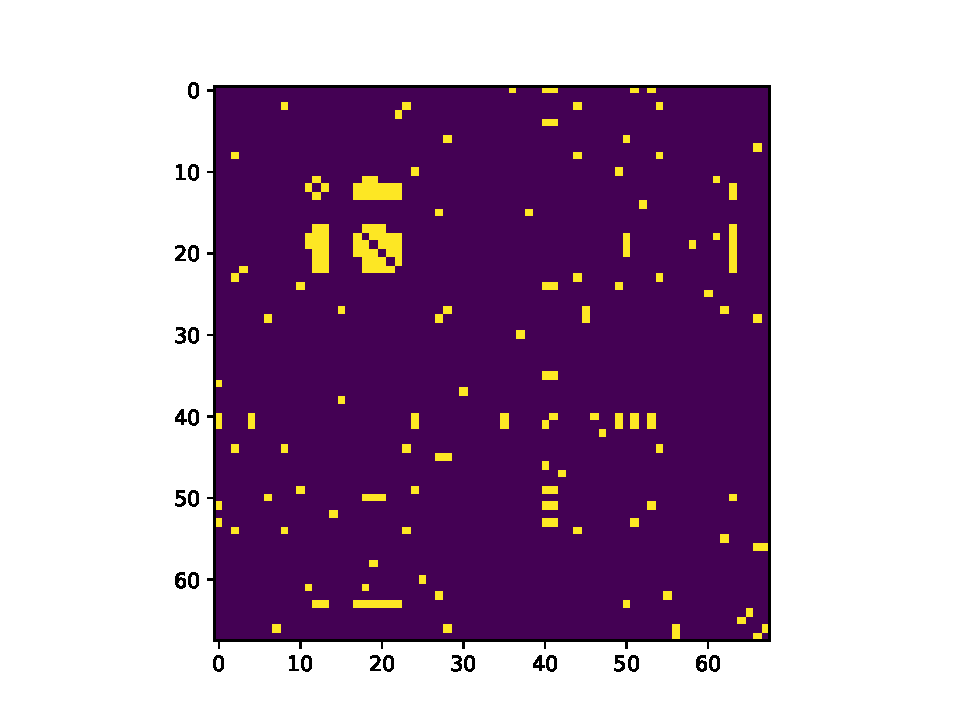
\includegraphics[width=.5\linewidth]{../figures/DrySeeds.pdf}}
\subfloat[\centering Six-hour Imbibed]{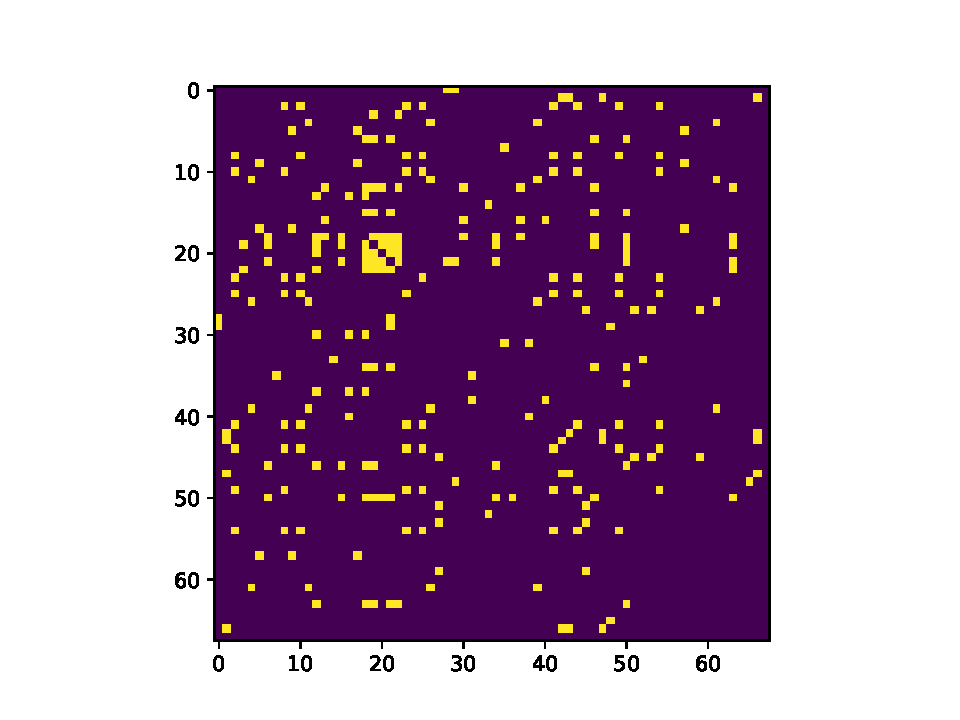
\includegraphics[width=.5\linewidth]{../figures/SixHourImbibed.pdf}}
\caption{Bitmap representation of the connectivity among metabolites.}\label{tomatos1}
\end{figure}

Figure \ref{tomatos2} shows the cluster which contains the GABA metabolite in both groups. Both clusters are highly connected, but in the Dry Seed group (left) the cluster consists of five metabolites, whereas in the Six-hour Imbibed group four additional metabolites are found to be in the GABA cluster. All the edges in Figure \ref{tomatos2}(a) are also detected to be present in Figure \ref{tomatos2}(b). 

\begin{figure}[t!]
\centering
\subfloat[\centering Dry Seeds]{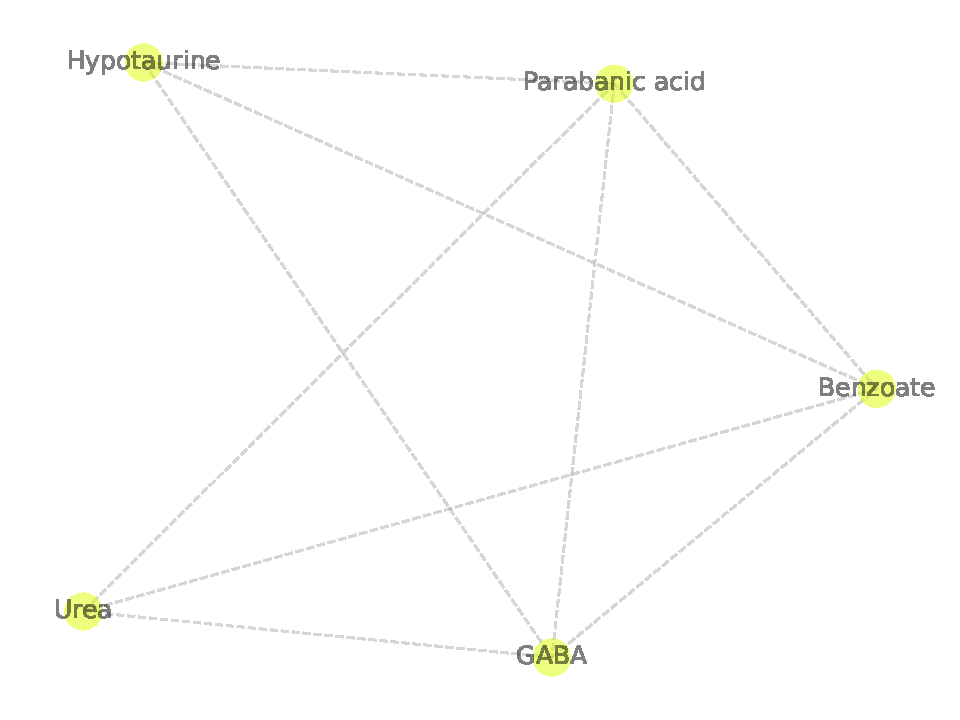
\includegraphics[width=.45\linewidth]{../figures/Gaba0.pdf}}
\subfloat[\centering Six-hour Imbibed]{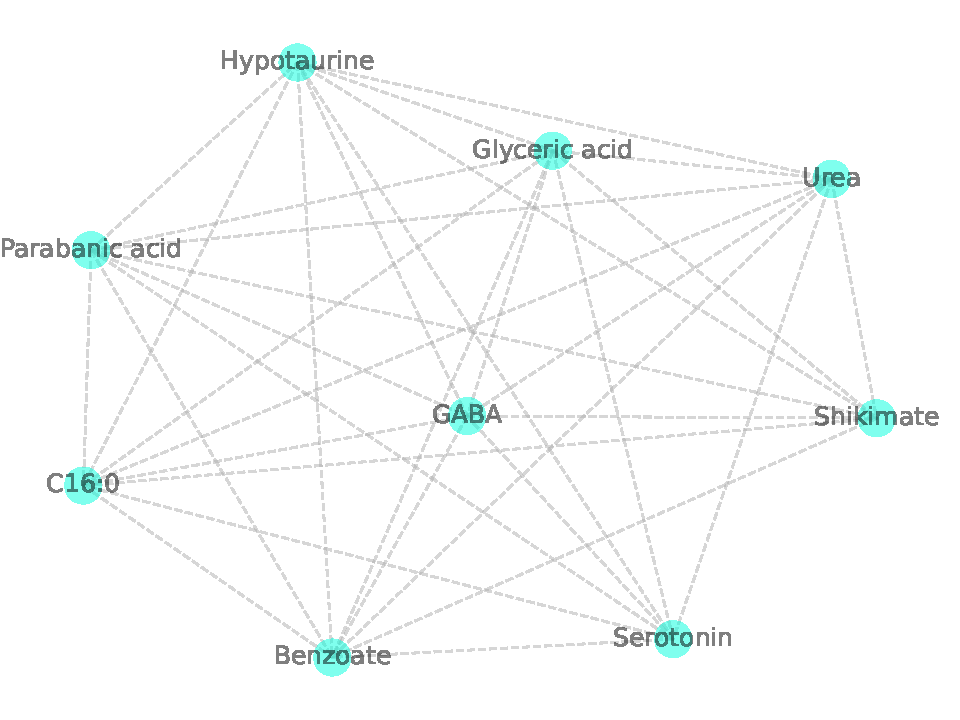
\includegraphics[width=.45\linewidth]{../figures/Gaba1.pdf}}
\caption{The network component containing the GABA metabolite in each group.}\label{tomatos2}
\end{figure}


\bibliographystyle{abbrvnat}

\begin{thebibliography}{99}

\bibitem{Frankl1990}
Peter Frankl and Hiroshi Maehara.
\newblock Some geometric applications of the beta distribution.
\newblock \emph{Annals of the Institute of Statistical Mathematics},
  42:\penalty0 463--474, 1990.

\bibitem{tomatos2017}
Rashid Kazmi, Leo Willems, Ronny Joosen, Noorullah Khan, Wilco Ligterink, and
  Henk Hilhorst.
\newblock Metabolomic analysis of tomato seed germination.
\newblock \emph{Metabolomics}, 13, 12 2017.
\newblock doi{10.1007/s11306-017-1284-x}.

\end{thebibliography}

\end{document}          
